\lecture{12}{2025-10-17}{}{}
What we want now is to go back to memory and spent quite a lot of time on this topic. What we will change here is that we will care about the performance of the memory we are building.

\section{Caches}
The question we have is what is the problem with memory:
\begin{center}
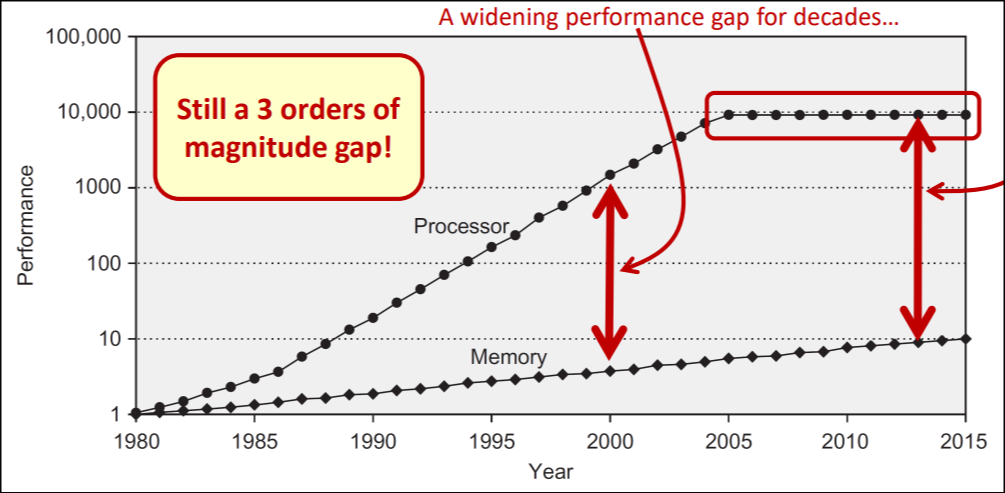
\includegraphics[scale=0.2]{screenshots/2025-10-17_6.png}
\end{center}
Processor has been improved a \important{lot} in comparisaison of memory. What memory means here is DRAM.\\
The issue is that we want a big memory and a fast processor which cannot really work well together, we need to \important{so something} ourself.\\
What we can do is to use other type of memory which is \important{faster but expensive} 
\begin{tikzpicture}[
    box/.style = {draw, minimum width=2.8cm, minimum height=1cm, align=center, font=\small},
    label/.style = {font=\footnotesize, align=center}
  ]

  % Processor node
  \node[box] (processor) {Processor};

  % Child nodes
  \node[box, below left=of processor, xshift=-1.5cm] (dram) {DRAM};
  \node[box, below=of processor] (sram1) {SRAM};
  \node[box, below right=of processor, xshift=1.5cm] (sram2) {SRAM};
  \node[box, below=of sram2, yshift=-0.8cm] (sram3) {SRAM};

  % Arrows from processor to memory
  \draw[->] (processor) -- (dram);
  \draw[->] (processor) -- (sram1);
  \draw[->] (processor) -- (sram2);
  \draw[->] (sram2) -- (sram3);

  % Annotations
  \node[label, below=0.1cm of dram] {30--50ns\\10--100GB};
  \node[label, below=0.1cm of sram1] {10--20ns\\1--10MB};
  \node[label, below=0.1cm of sram2] {3--10ns\\100KB};
  \node[label, below=0.1cm of sram3] {$<$1ns\\10KB};

\end{tikzpicture}


\begin{center}
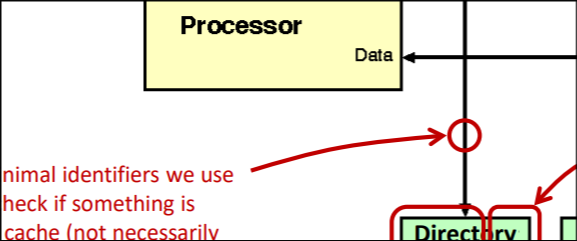
\includegraphics[scale=0.3]{screenshots/2025-10-17_7.png}
\end{center}


So the fact is: this is not only a technology issue even though we are not able to make \texttt{DRAM} faster. It's not even an issue with \texttt{SRAM} cost, it wouldn't be too costly to make \texttt{SRAM} bigger, the issue is that even though SRAM is pretty maleable, when expanding it, it becomes 2 to 3 degree of magnitude slower (in terms of clock cycles).

\begin{parag}{What memory to use?} The question is where do we put our data, in which memory.\\
	For instance let us took a look at this code:
	\begin{lstlisting}[langage=c]
i = 0;
sum = 0;
while (i < 1024) {
	sum = sum + a[i];
	i = i + 1; 
}
	\end{lstlisting}
	
	\begin{itemize}
	    \item Intruction corresponds to line 3-5 that are \important{read over and over}should be in fast memory
	    \item if variable \texttt{i} and \texttt{sum} are stored in memory, they are also \important{used often} and should be stored in fast memory
	    \item One would like to anticipate the future and load the \important{following} instructions and vector elements.
	\end{itemize}
\end{parag}
\begin{parag}{Spatial and Temporal locality}
    There is two important criteria for the choice of the placement:
	\begin{itemize}
	    \item \textbf{Temporal locality}
			\begin{itemize}
			    \item Data that have been \important{used recently}, have likelyhood of being used again (Code: loop, function, ...) (Data: local variables and data structures)
			\end{itemize}
			\item Spatial locality
				\begin{itemize}
				    \item Data which \important{follow in the memory other data} that are currently used are likelyhood to be used in the future (Code are usually sequential, Data: array)
				\end{itemize}
	\end{itemize}
	However, this is not perfect, this is onlyl a probablistic model. We are only making guess and hoping there were right so that we can win some time.
\end{parag}

\begin{parag}{Our placment policy most be:}
    \begin{subparag}{Invisible to the programmer}
        \begin{itemize}
            \item One could analyse data structures and program semantics to detect heabily used vairables/arrays and thus decide placment $\to$ OK in some context (emebedded) but we want to have the programmers not to go through this hassle 
            \item To do so, we will add \important{hardware} to help
        \end{itemize}
    \end{subparag}
	\begin{subparag}{Extremly simple and fast}
		The decision are made in the hardware, they need to be simple. The goal is to accesst memory very fast, in the order of a ns or less:  \important{not much time} to make a complex decision...
	\end{subparag}
\end{parag}


\subsubsection{Cache: The idea}
The main difference between this and the tree make before is that now as a \important{programmer} I don't know which memory I am using, I am at a level of abstraction above which makes it easier for me to develop software.\\
The idea behind the cache is the fololowing:\\
The processor makes a request for an address, we first check if the address is in the dirc


